%! Author = joels
%! Date = 31/01/2022

\section{Code-Analyse}
\begin{itemize}[topsep=0pt]
    \itemsep -0.2em
    \item Mächtige generische Code-Analyse-Technik
    \item Für viele Optimierungen nützlich
\end{itemize}

\subsection{Control Flow Graph (CFG)}
\begin{itemize}[topsep=0pt]
    \itemsep -0.2em
    \item Repräsentiert alle möglichen Programmpfade
    \item Propagiere Informationen durch den Graph, bis es stabil ist
    \item Knoten = Basic Block
    \SubItem{Ununterbrochener Code-Abschnitt}
    \SubItem{Einstieg nur am Anfang: Kein Label in der Mitte}
    \SubItem{Ausstieg nur am schluss: Kein Branch in der Mitte}
    \item Kante
    \SubItem{Bedingter oder unbedingter Branch}
\end{itemize}
\begin{minipage}{0.6\linewidth}
    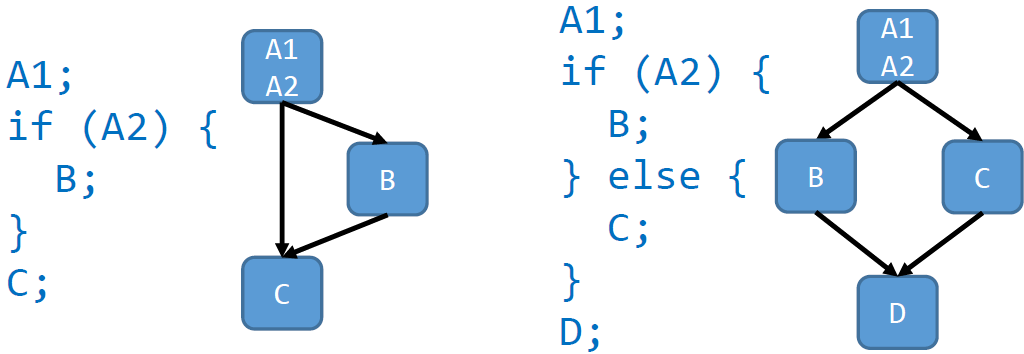
\includegraphics[width=\linewidth]{cfg_if}
\end{minipage}
\begin{minipage}{0.4\linewidth}
    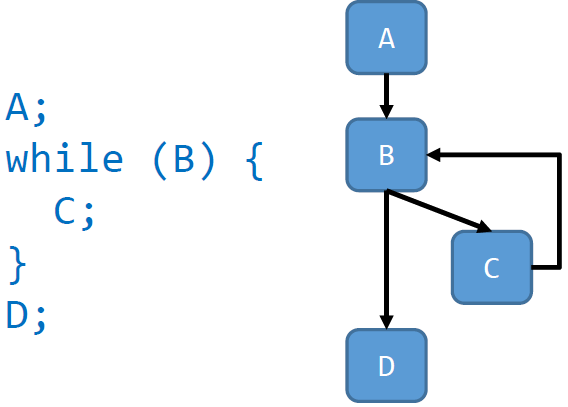
\includegraphics[width=\linewidth]{cfg_while}
\end{minipage}

\subsection{Dataflow Analysis}
\begin{minipage}{0.5\linewidth}
    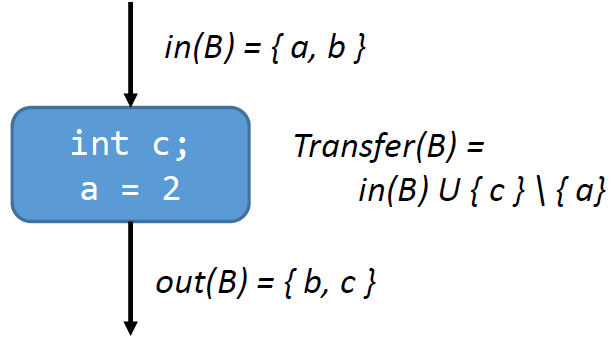
\includegraphics[width=\linewidth]{cfg_transfer}
\end{minipage}
\begin{minipage}{0.5\linewidth}
    $\rightarrow$ Fixpunkt-Iteration über CFG bis jeder Block stabil ist.\\
    \textbf{State:} Menge der uninitialisierten Variablen\\
    Input und Output State pro Basic Block. AnalyseInformationen vor und nach einem Block.\\
    \textbf{Transfer:} Füge Deklarationen dazu, entferne zugewiesene Variablen\\
\end{minipage}

\begin{lstlisting}
boolean stable;
do {
    stable = true;
    for (var block : graph.allBlocks()) {
        in[block] = join(block.predecessors().outStates());
        var oldOut = out[block];
        out[block] = transfer (in[block]);
        if (!out[block].equals(oldOut)) {
            stable = false;
        }
    }
} while (!stable);
\end{lstlisting}

\subsection{Diskussion}
\begin{itemize}[topsep=0pt]
    \itemsep -0.2em
    \item Konservative Analyse
    \SubItem{Betrachtet alle möglichen syntaktischen Pfade}
    \item Kontextfreie Analyse
    \SubItem{Alle Pfade werden gewählt, egal ob Bedingung erfüllt ist}
    \item Fehlermeldung ist auch konservativ
    \SubItem{Falls mindestens ein Pfad mit Fehler existiert $\rightarrow$ Error}
    \item Fixpunkt-Iteration muss terminieren
    \SubItem{Z.B. falls Menge monoton mit Joins wächst}
\end{itemize}

\subsection{Andere Anwendungen}
\begin{itemize}[topsep=0pt]
    \itemsep -0.2em
    \item Constant Propagation
    \SubItem{Konstante Werte bei Transfer merken}
    \SubItem{Join = Intersection}
    \item Rückwärts-Propagierung
    \SubItem{Transfer: Out State $\rightarrow$ In State}
    \SubItem{Z.B. für Dead Code Analysis}
\end{itemize}